\documentclass[10pt]{article}
\usepackage[ngerman]{babel}
\usepackage[utf8]{inputenc}
\usepackage[T1]{fontenc}
\usepackage{hyperref}
\hypersetup{colorlinks=true, linkcolor=blue, filecolor=magenta, urlcolor=cyan,}
\urlstyle{same}
\usepackage{graphicx}
\usepackage[export]{adjustbox}
\graphicspath{ {./images/} }
\usepackage{amsmath}
\usepackage{amsfonts}
\usepackage{amssymb}
\usepackage[version=4]{mhchem}
\usepackage{stmaryrd}

\author{SuiWeb: JSX, SJDON\\
demo-01-jsx.html\\
demo-01-sjdon.html\\
Didact: (Rodrigo Pombo)\\
https://codesandbox.io/s/didact-2-k6rbj?file=/src/index.js}
\date{}


\begin{document}
\maketitle
\section*{WBE: Ul-BIBLIOTHEK}
 TEIL 2: IMPLEMENTIERUNG\section*{ÜBERSICHT}
\begin{itemize}
  \item Interne Repräsentation und das DOM
  \item Komponenten und Properties
  \item Darstellung von Komponenten
  \item Defaults und weitere Beispiele
\end{itemize}

\section*{ÜBERSICHT}
\begin{itemize}
  \item Interne Repräsentation und das DOM
  \item Komponenten und Properties
  \item Darstellung von Komponenten
  \item Defaults und weitere Beispiele
\end{itemize}

\section*{RÜCKBLICK}
\begin{itemize}
  \item Ziel: eigene kleine Bibliothek entwickeln
  \item Komponentenbasiert und datengesteuert
  \item An Ideen von React.js und ähnlicher Systeme orientiert
  \item Motto: „Keep it simple!"
  \item Bezeichnung:
\end{itemize}

\section*{SuiWeb}
Simple User Interface Toolkit for Web Exercises

\section*{RÜCKBLICK}
\begin{itemize}
  \item Notation für den Aufbau der Komponenten
  \item JSX: in React.js verwendet
  \item SJDON: eigene Notation
  \item SuiWeb soll beide Varianten unterstützen
\end{itemize}

\begin{verbatim}
// jsx
const element = (<h1 title="foo">Hello</h1>)
// sjdon
const element = ["h1", {title: "foo"}, "Hello"]
\end{verbatim}

\section*{ANSTEHENDE AUFGABEN}
\begin{itemize}
  \item Interne Repräsentation der Komponenten
  \item Konvertierung von JSX und SJDON in diese Repräsentation
  \item Abbildung interne Repräsentation ins DOM
  \item Daten steuern Komponenten: Properties
  \item Hierarchie von Komponenten
  \item Komponenten mit Zustand
\end{itemize}

Anregungen und Code-Ausschnitte aus:\\
Rodrigo Pombo: Build your own React\\
\href{https://pomb.us/build-your-own-react/}{https://pomb.us/build-your-own-react/}\\
Zachary Lee: Build Your Own React.js in 400 Lines of Code \href{https://webdeveloper.beehiiv.com/p/build-react-400-lines-code}{https://webdeveloper.beehiiv.com/p/build-react-400-lines-code}

\section*{AUSGANGSPUNKT}
\begin{verbatim}
// jsx
/** @jsx createElement */
const element = (<h1 title="foo">Hello</h1>)
// jsx babel output (React < 17)
const element = createElement(
    "h1",
    { title: "foo" },
    "Hello"
)
// sjdon
const element = ["h1", {title: "foo"}, "Hello"]
\end{verbatim}

\section*{INTERNE REPRÄSENTATION}
\begin{verbatim}
// jsx babel output
const element = createElement(
    "h1",
    { title: "foo" },
    "Hello"
)
\end{verbatim}

\begin{verbatim}
// internal representation
const element = {
    type: "h1",
    props: {
        title: "foo",
        children: ["Hello"],
    },
}
\end{verbatim}

\section*{INTERNE REPRÄSENTATION}
\begin{verbatim}
{
    type: "h1",
    props: {
        title: "foo",
        children: ["Hello"], /* noch anzupassen */
    },
}
\end{verbatim}

\begin{itemize}
  \item Element: Objekt mit zwei Attributen, type und props
  \item type: Name des Elements ("body", "h1", ...)
  \item props: Attribute des Elements
  \item props.children: Kindelemente (Array)
\end{itemize}

\section*{TEXT-ELEMENT}
\begin{verbatim}
{
    type: "TEXT_ELEMENT",
    props: {
        nodeValue: "Hello",
        children: [],
    },
}
\end{verbatim}

\begin{itemize}
  \item Aufbau analog zu anderen Elementen
  \item Spezieller Typ: "TEXT\_eLEMENT"
\end{itemize}

\section*{VERSCHACHTELTE ELEMENTE}
\begin{center}
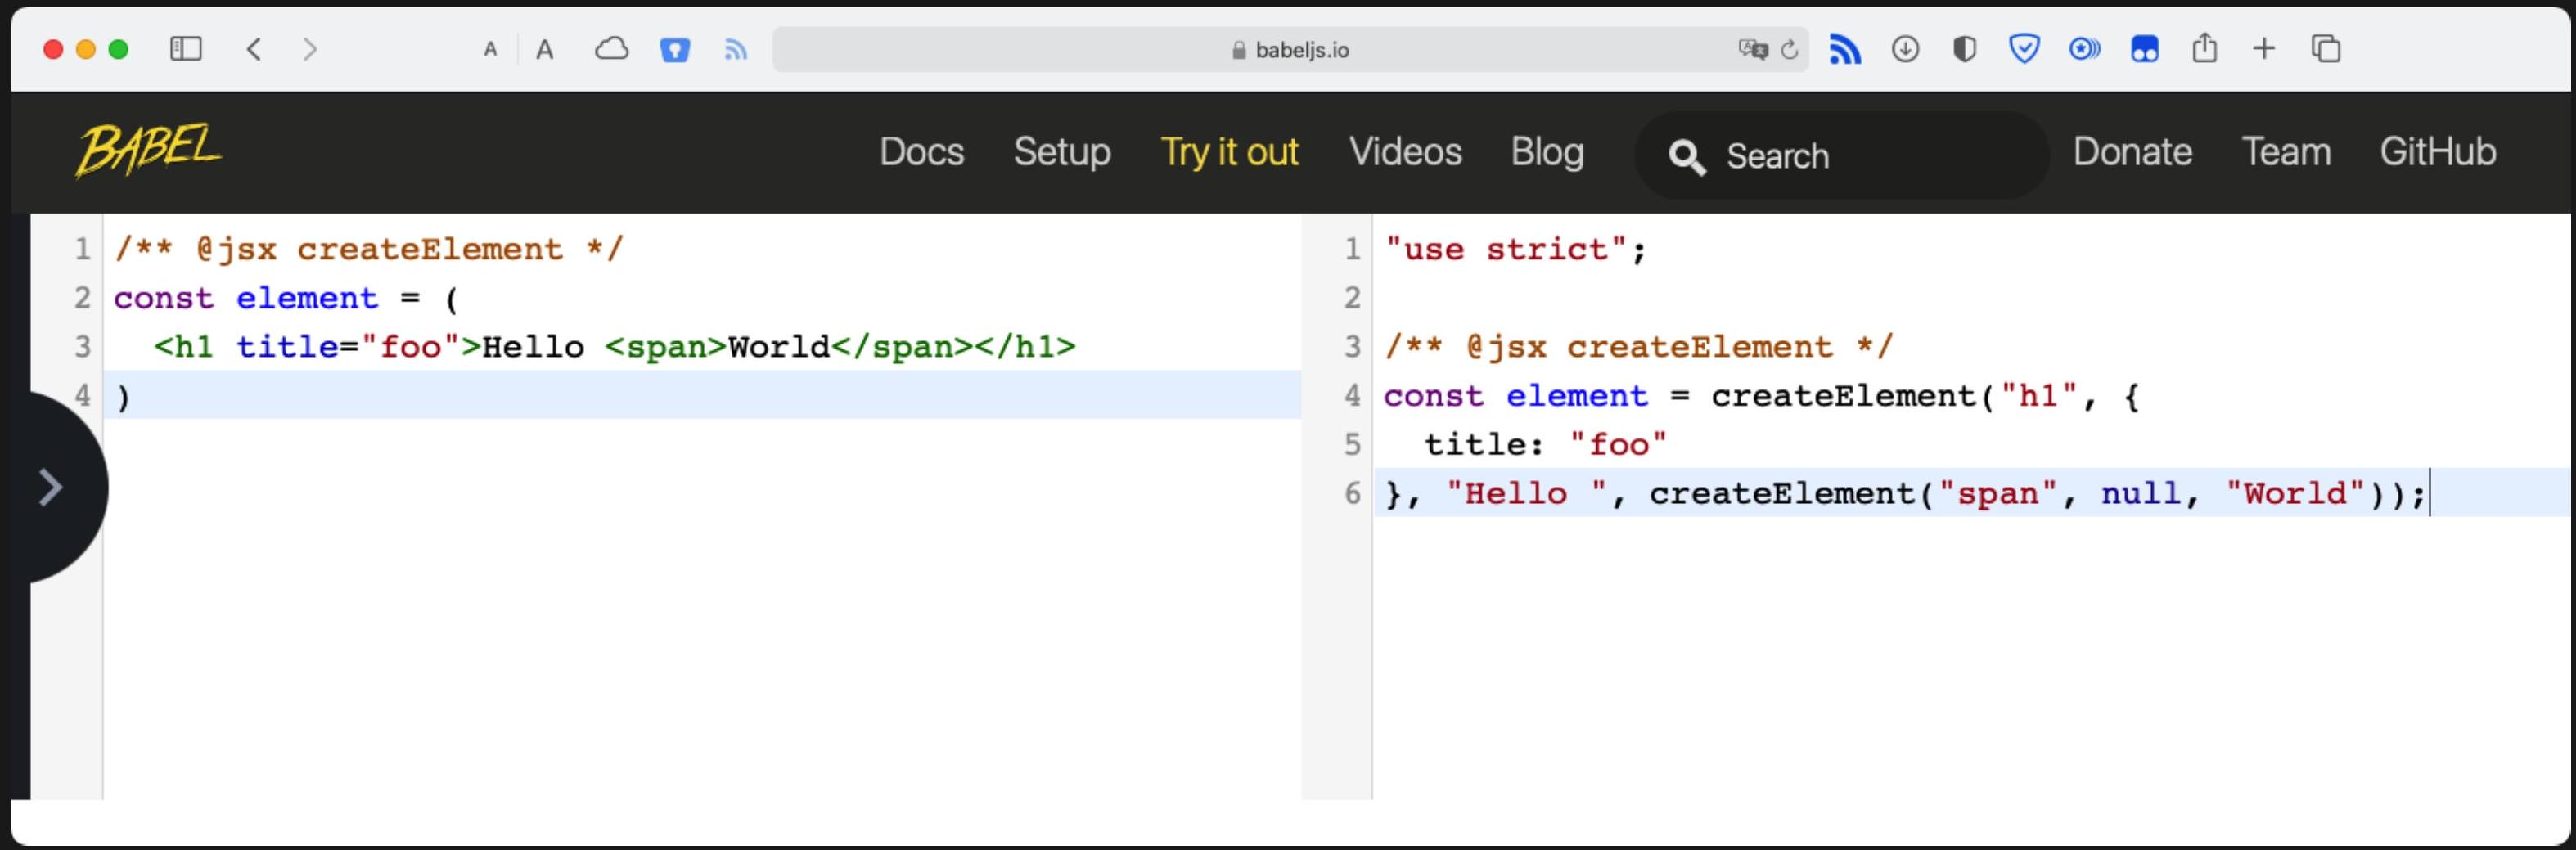
\includegraphics[width=\linewidth]{images/2025_01_02_254b5e4c52d090c313e1g-11}
\end{center}

\begin{itemize}
  \item Mehrere Kindelemente: ab drittem Argument von createElement
  \item Verschachtelte Elemente: rekursive Aufrufe von createElement
\end{itemize}

\section*{KONVERTIERUNG VON JSX}
\begin{verbatim}
function createElement (type, props,
                                ...children) {
    return {
        type,
        props: {
            ...props,
            children: children.map(child =>
                typeof child === "object"
                    ? child
                : createTextElement(child)
            ),
    },
    }
}
\end{verbatim}

\begin{verbatim}
function createTextElement (text) {
    return {
        type: "TEXT_ELEMENT",
        props: {
            nodeValue: text,
            children: [],
        },
    }
}
\end{verbatim}

\section*{CREATEELEMENT: BEISPIEL}
\begin{verbatim}
// <div>Hello<br></div>
createElement("div", null, "Hello", createElement("br", null))
// returns
{
    type: 'div',
    props: {
        children: [
            {
                type: 'TEXT_ELEMENT',
                    props: { nodeValue: 'Hello', children: [] }
            },
            { type: 'br', props: { children: [] } }
        ]
    }
}
\end{verbatim}

\section*{KONVERTIERUNG VON SJDON}
\begin{verbatim}
function parseSJDON ([type, ...rest]) {
    const isObj = (obj) => typeof(obj)==='object' && !Array.isArray(obj)
    const children = rest.filter(item => !isObj(item))
    return createElement(type,
        Object.assign({}, ...rest.filter(isObj)),
        ...children.map(ch => Array.isArray(ch) ? parseSJDON(ch) : ch)
    )
}
\end{verbatim}

\begin{itemize}
  \item Abbildung auf createElement-Funktion
  \item Attribute in einem Objekt zusammengeführt
  \item Kindelemente bei Bedarf (Array) ebenfalls geparst
\end{itemize}

\section*{ZWISCHENSTAND}
\begin{itemize}
  \item Einheitliche Repräsentation für Elemente unabhängig von der ursprünglichen Syntax (JSX or SJDON)
  \item Baumstruktur von Elementen
  \item Text-Elemente mit leerem Array children
  \item DOM-Fragment im Speicher repräsentiert (virtuelles DOM?)
\end{itemize}

Zu tun:

\begin{itemize}
  \item Abbildung der Baumstruktur ins DOM
\end{itemize}

\section*{RENDER TO DOM}
\begin{verbatim}
function render (element, container) {
    /* create DOM node */
    const dom =
        element.type == "TEXT_ELEMENT"
            ? document.createTextNode("")
            : document.createElement(element.type)
    /* assign the element props */
    const isProperty = key => key !== "children"
    Object.keys(element.props)
        .filter(isProperty)
        .forEach(name => { dom[name] = element.props[name] })
    /* render children */
    element.props.children.forEach(child => render(child, dom))
    /* add node to container */
    container.appendChild(dom)
}
\end{verbatim}

\section*{HTML-ELEMENTE}
\begin{itemize}
  \item Komponenten können HTML-Elemente verwenden
  \item Tagnamen in Kleinbuchstaben
  \item Gross-/Kleinschreibung ist relevant
  \item Übliche Attribute für HTML-Elemente möglich
  \item Wenig Ausnahmen: className statt class
\end{itemize}

\section*{BEISPIEL}
\begin{center}
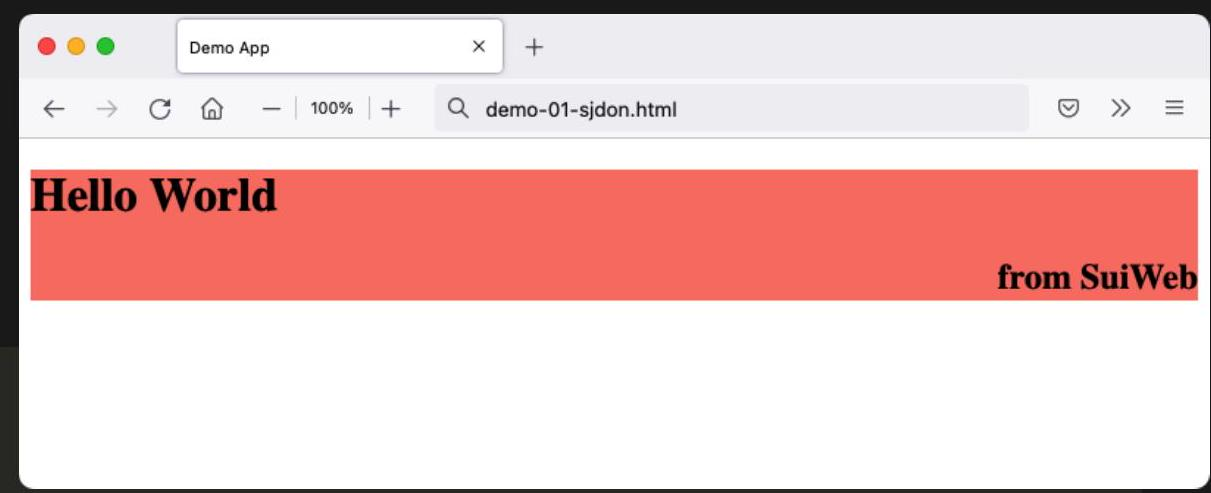
\includegraphics[width=\linewidth]{images/2025_01_02_254b5e4c52d090c313e1g-18}
\end{center}

\begin{verbatim}
import { render } from "./lib/suiweb-1.1.js"
const element =
    ["div", {style: "background:salmon"},
        ["h1", "Hello World"],
        ["h2", {style: "text-align:right"}, "from SuiWeb"] ]
const container = document.getElementById("root")
render(element, container)
\end{verbatim}

\section*{ZWISCHENSTAND}
\begin{itemize}
  \item Interne Struktur aufbauen
  \item Ins DOM rendern
\end{itemize}



\section*{ÜBERSICHT}
\begin{itemize}
  \item Interne Repräsentation und das DOM
  \item Komponenten und Properties
  \item Darstellung von Komponenten
  \item Defaults und weitere Beispiele
\end{itemize}

\section*{FUNKTIONSKOMPONENTEN}
\begin{verbatim}
1 const App = (props) =>
    ["h1", "Hi ", props.name]
4 const element =
5 [App, {name: "foo"}]
\end{verbatim}

\begin{itemize}
  \item App ist eine Funktionskomponente
  \item Die zugehörige Repräsentation erzeugt keinen DOM-Knoten
  \item Ergebnis des Aufrufs liefert auszugebende Struktur
  \item Konvention: eigene Komponenten mit grossen Anfangsbuchstaben
\end{itemize}

\section*{PROBLEM}
\begin{itemize}
  \item Komponenten in JSX retournieren mittels createElement erzeugte interne Strukturen
  \item Unter SJDON liefern sie allerdings SJDON-Code, der nach Aufruf der Komponente noch geparst werden muss
  \item Abhilfe: SJDON-Komponenten erhalten ein Attribut sjdon, welches die Konvertierung (parseSJDON ) ergänzt
  \item Dieses Attribut lässt sich mit einer kleinen Hilfsfunktion anbringen
\end{itemize}

\section*{SJDON-KONVERTIERUNG ERWEITERT}
\begin{verbatim}
function useSJDON (...funcs) {
    for (let f of funcs) {
        const fres = (...args) => parseSJDON(f(...args))
        f.sjdon = fres
    }
}
\end{verbatim}

\begin{itemize}
  \item Kann für mehrere Komponentenfunktionen aufgerufen werden, indem sie als Argumente übergeben werden
  \item Diese werden um das sjdon-Attribut ergänzt
\end{itemize}

\section*{FUNKTIONSKOMPONENTEN}
\begin{itemize}
  \item Funktion wird mit props-Objekt aufgerufen
  \item Ergebnis ggf. als SJDON geparst
\end{itemize}

\begin{verbatim}
switch (typeof type)
    case 'function': {
        let children
        if (typeof(type.sjdon) === 'function') {
            children = type.sjdon(props)
        } else {
            children = type(props)
        }
        reconcileChildren(...)
        break
    }
}
\end{verbatim}

\section*{BEISPIEL}
\begin{verbatim}
const App = (props) =>
    ["h1", {style: "background: mediumaquamarine"}, "Hi ", props.name]
const element =
    [App, {name: "SuiWeb"}]
// notify SuiWeb that the App component returns SJDON
useSJDON(App)
const container = document.getElementById ©\bullet. Domonop
render(element, container)
demo-02-jsx.html demo-02-sjdon.html
\end{verbatim}

\begin{center}
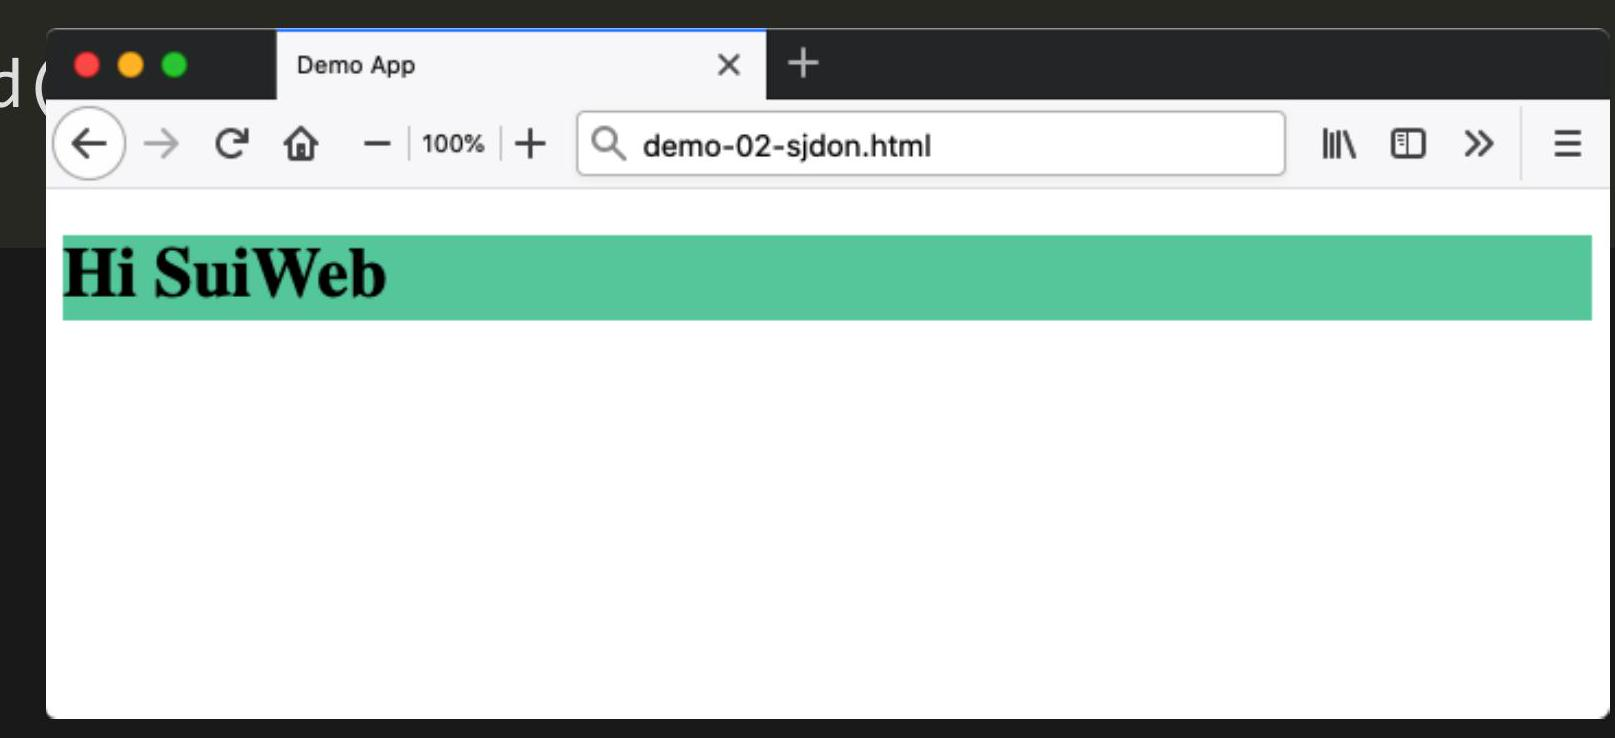
\includegraphics[width=\linewidth]{images/2025_01_02_254b5e4c52d090c313e1g-25}
\end{center}

\section*{WERTE STEUERN UI-AUFBAU}
\begin{verbatim}
const App = () => {
    const enabled = false
    const text = 'A Button'
    const placeholder = 'input value...'
    const size = 50
    return (
        ["section",
            ["button", {disabled: !enabled}, text],
            ["input", {placeholder, size, autofocus: true}] ]
    )
}
\end{verbatim}

demo-03-values

\section*{ARRAY ALS LISTE AUSGEBEN}
\begin{verbatim}
const List = ({items}) =>
    ["ul", ...items.map((item) => ["li", item]) ]
const element =
    [List, {items: ["milk", "bread", "sugar"]}]
useSJDON(List)
\end{verbatim}

\begin{itemize}
  \item Die props werden als Argument übergeben
  \item Hier interessiert nur das Attribut items\\
demo-04-liste
\end{itemize}

\section*{OBJEKT ALS TABELLE}
\begin{verbatim}
const ObjTable = ({obj}) =>
    ["table", {style},
        ...Object.keys(obj).map((key) =>
        ["tr", ["td", key], ["td", obj[key]]])]
const style = {
    width: "8em",
    background: "lightblue",
}
const element =
    [ObjTable, {obj: {one: 1111, two: 2222, three: 3333}}]
demo-05-object
\end{verbatim}

\section*{VERSCHACHTELN VON ELEMENTEN}
\begin{verbatim}
/* JSX */
<MySection>
    <MyButton>My Button Text</MyButton>
</MySection>
\end{verbatim}

\begin{itemize}
  \item Eigene Komponenten können verschachtelt werden
  \item MyButton ist mit seinem Inhalt in props.children von MySection enthalten
\end{itemize}

\section*{VERSCHACHTELN VON ELEMENTEN}
\begin{verbatim}
const MySection = ({children}) =>
    ["section", ["h2", "My Section"], ...children]
const MyButton = ({children}) =>
    ["button", ...children]
const element =
    [MySection, [MyButton, "My Button Text"]]
useSJDON(MyButton, MySection)
\end{verbatim}

demo-06-nested

\section*{TEILBÄUME WEITERGEBEN}
\begin{verbatim}
const Main = ({header, name}) =>
    ["div",
        [...header, name],
        ["p", "Welcome to SuiWeb"] ]
const App = ({header}) =>
    [Main, {header, name: "web developers"}]
const element = [App, {header: ["h2", "Hello "]}]
useSJDON(App, Main)
\end{verbatim}

demo-07-subtree

\section*{ÜBERSICHT}
\begin{itemize}
  \item Interne Repräsentation und das DOM
  \item Komponenten und Properties
  \item Darstellung von Komponenten
  \item Defaults und weitere Beispiele
\end{itemize}

\section*{DARSTELLUNG}
\begin{itemize}
  \item Komponenten müssen ggf. mehrere Styles mischen können
  \item Neben Default-Darstellung auch via props eingespeist
  \item Daher verschiedene Varianten vorgesehen:
  \item CSS-Stil als String
  \item Objekt mit Stilangaben
  \item Array mit Stil-Objekten
\end{itemize}

\section*{DARSTELLUNG}
\begin{verbatim}
function combineStyles (styles) {
    let styleObj = {}
    if (typeof(styles)=="string") return styles
    else if (Array.isArray(styles)) styleObj = Object.assign({}, ...styles)
    else if (typeof(styles)=="object") styleObj = styles
    else return ""
    let style = ""
    for (const prop in styleObj) {
        style += prop + ":" + styleObj[prop] + ";"
    }
    return style.replace(/([a-z])([A-Z])/g, "$1-$2").toLowerCase()
}
\end{verbatim}

\section*{BEISPIEL}
\begin{verbatim}
const StyledList = ({items}) => {
    let style = [styles.listitem, {color: "#556B2F"}]
    return (
        ["ul", ...items.map((item) => ["li", {style}, item]) ]
    )
}
const element =
    [StyledList, {items: ["milk", "bread", "sugar"]}]
const styles = {
    listitem: {
            padding: "1em",
            margin: "0.5em 2em",
            fontSize: "1.5em",
            ... }
}
\end{verbatim}

\begin{center}
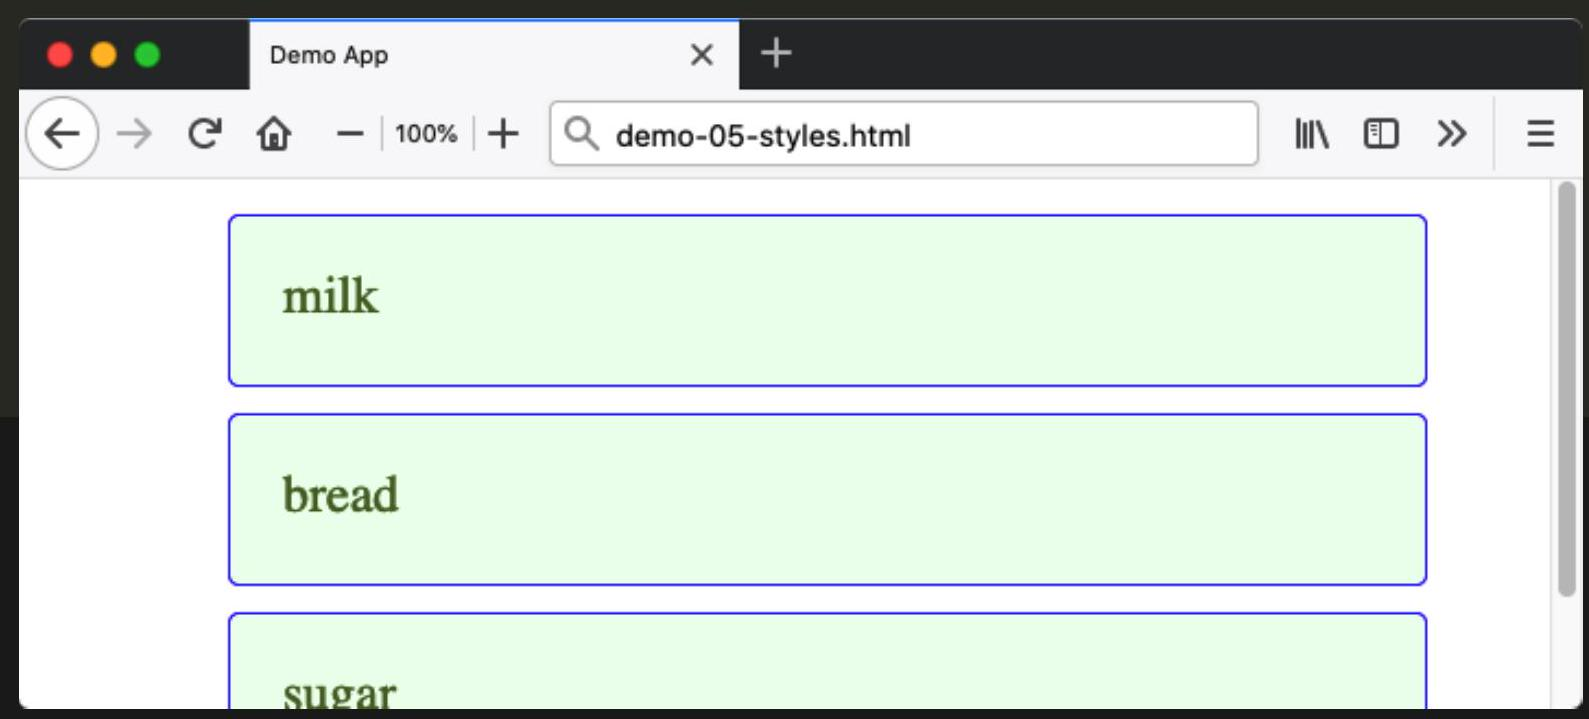
\includegraphics[width=\linewidth]{images/2025_01_02_254b5e4c52d090c313e1g-35}
\end{center}

\section*{ÜBERSICHT}
\begin{itemize}
  \item Interne Repräsentation und das DOM
  \item Komponenten und Properties
  \item Darstellung von Komponenten
  \item Defaults und weitere Beispiele
\end{itemize}

\section*{DEFAULT PROPERTIES}
\begin{verbatim}
const App = () => (
        ["main",
            [MyButton, {disabled: true, text: 'Delete'}],
            [MyButton] ]
)
const MyButton = ({disabled=false, text='Button'}) => (
    ["button", disabled ? {disabled} : {}, text]
)
\end{verbatim}

demo-09-defaultprops

\section*{DEFAULT PROPERTIES}
\begin{itemize}
  \item Übergebene Properties überschreiben Defaults
  \item Selbst zu implementieren (ist einfach, s. Beispiel)
  \item In React.js können Defaults an Funktion gehängt werden: (in SuiWeb nicht umgesetzt, wäre aber möglich)
\end{itemize}

\begin{verbatim}
const MyButton = (props) => { ... }
MyButton.defaultProps = {
    text: 'My Button',
    disabled: false,
}
\end{verbatim}

\section*{WEITERES BEISPIEL}
\begin{verbatim}
const MyButton = ({children, disabled=true}) =>
    ["button", {style: "background: khaki", disabled}, ...children]
const Header = ({name, children}) =>
    ["h2", "Hello ", name, ...children]
const App = (props) =>
    ["div",
        [Header, {name: props.name}, " and", ["br"], "web developers"],
        [MyButton, "Start", {disabled:false}],
        [MyButton, "Stop"] ]
useSJDON(App, Header, MyButton)
render([App, {name: "SuiWeb"}], container)
\end{verbatim}

demo-10-children

\section*{ZAHLEN IN PROPS}
\begin{verbatim}
const App = ({num1, num2}) =>
    ["h1", num1, " * ", num2, " = ", num1*num2]
const element = [App, {num1: 3, num2: 9}]
\end{verbatim}

\begin{itemize}
  \item Beim Funktionsaufruf als Zahlen behandelt
  \item Beim Rendern in Textknoten abgelegt\\
demo-11-numbers\\
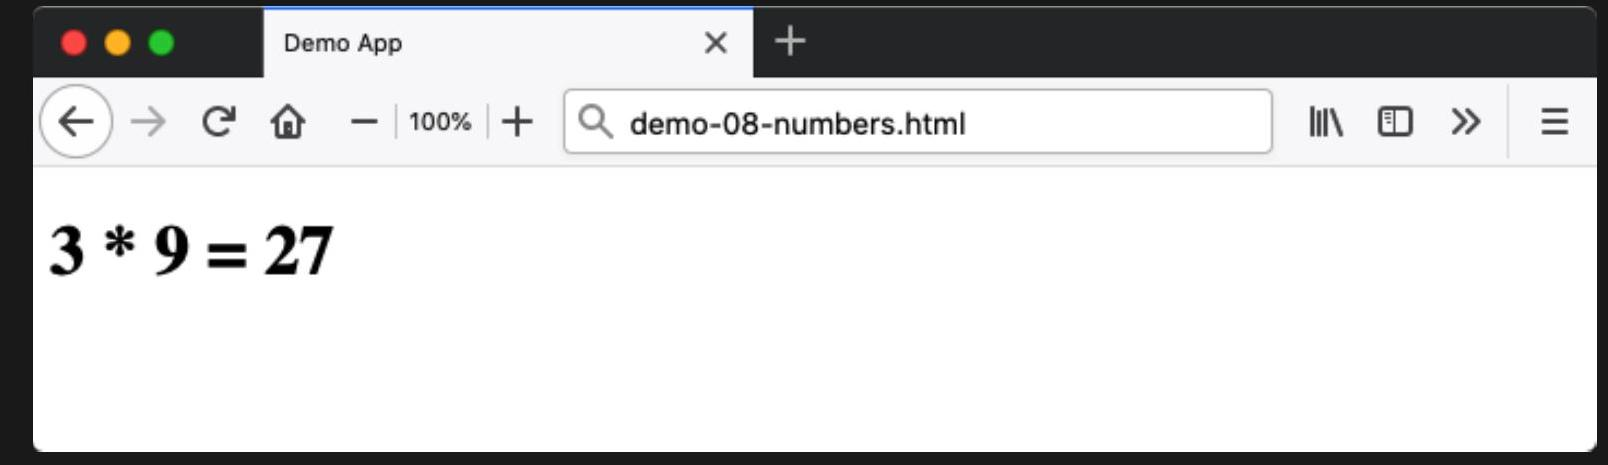
\includegraphics[width=\linewidth]{images/2025_01_02_254b5e4c52d090c313e1g-40}
\end{itemize}

\section*{AKTUELLER STAND}
\begin{itemize}
  \item Notationen, um Komponenten zu definieren: JSX, SJDON
  \item Funktionen zur Anzeige im Browser: render-Funktion
  \item Daten können Komponenten steuern: Argument props
  \item Ausserdem: Verarbeiten von Styles, Default-Properties
  \item Also: Ul-Aufbau mit Komponenten
  \item Was noch fehlt: Mutation, Zustand\\
$\rightarrow$ nächste Woche :)
\end{itemize}

\section*{VERWEISE}
\begin{itemize}
  \item Build Your Own React.js in 400 Lines of Code \href{https://webdeveloper.beehiiv.com/p/build-react-400-lines-code}{https://webdeveloper.beehiiv.com/p/build-react-400-lines-code}
  \item Rodrigo Pombo: Build your own React \href{https://pomb.us/build-your-own-react/}{https://pomb.us/build-your-own-react/}
  \item SuiWeb - An Educational Web Framework (Inspired by React) \href{https://github.com/suiweb/suiweb}{https://github.com/suiweb/suiweb}
\end{itemize}

\section*{Stand:}
7.12.2024 12:51


\end{document}